\textbf{ID:} UC13 (View Post) \\
\textbf{Scope:} CS Automated Information Timeline \\
\textbf{Level:} User goal \\
\textbf{Primary Actor:} Audience \\
\textbf{Stakeholders and Interests: }
\begin{itemize}
    \item Audience: A person that is interested in viewing all approved content on the system using their mobile device.
    \item Faculty: A person that works for the university and is interested in gaining visibility of their post and/or event.
    \item Office Manager: A person that works for the university and is interested in prioritizing the order of posts and/or events.
    \item Admin/Reviewer: A person that works for the university and approves and/or removes posts and/or events from the system.
\end{itemize}
\textbf{Preconditions: }
\begin{itemize}
    \item A post has been created and staged for display.
\end{itemize}
\textbf{Postconditions:} None \\
\textbf{Main Success Scenario: }
\begin{enumerate}
    \item User accesses the web application UI by scanning the QR code on the display board.
    \item System presents the web view with posts staged for display
\end{enumerate}
\textbf{Alternative Flows: } \\
a. At any time, system fails or becomes unresponsive and does not provide an error message
\begin{enumerate}
    \item User performs a hard refresh on the browser (ctrl + f5 or shift + reload)
    \item System reloads the editable view for the post
\end{enumerate}

\begin{figure}[H]
    \centering
    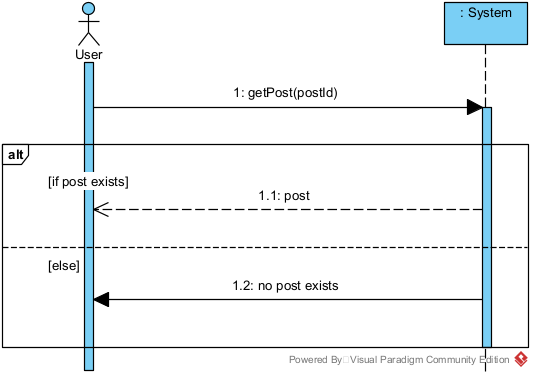
\includegraphics[width=0.8\textwidth]{images/SSD-UC13-ViewPost.png}
    \centering
    \caption{System Sequence Diagram: View Post}
\end{figure}

\textbf{Operation:} getPost(postId) \\
\textbf{Cross Reference:} UC13 (View Post)
\textbf{Preconditions:}
\begin{itemize}
    \item Post exists and is staged for display
    \item User is attempting to view a specific post (request)
\end{itemize}
\textbf{Postconditions:}
\begin{itemize}
    \item A PostService instance, postService  was created
    \item A PostRepository instance postRepository was created
    \item A Post instance post was created
    \item post was associated with the request
\end{itemize}